\section{Descripci\'on de la Implementaci\'on}
\label{sec:descripcion-implementacion}

En esta secci\'on se describen los detalles de la implementaci\'on de \foreign{TamTam Listens}.
Esto incluye la arquitectura y los componentes propios del sistema de reconocimiento del habla
los cuales, en conjunto con las herramientas mencionadas en las secciones anteriores, hacen posible
el funcionamiento de la interfaz mediante voz. 

\subsection{Arquitectura de TamTam Listens}
\label{sec:arquitectura-solucion}

La figura~\ref{figure:tamtam-listens-arq} muestra la arquitectura b\'asica de \emph{TamTam Listens}. Se 
pueden observar los componentes que forman parte de la soluci\'on desarrollada.

\begin{figure}[H] 
\centering

\includegraphics[width=0.7\textwidth]{./graphics/tamtam-listens-arq.png}
\caption{Arquitectura b\'asica de \emph{TamTam Listens}}
\label{figure:tamtam-listens-arq}
\end{figure}

Como sugiere la figura~\ref{figure:tamtam-listens-arq}, \emph{TamTam Listens} a\~nade soporte 
de reconocimiento del habla a \emph{TamTam Edit} utilizando la librer\'ia \emph{PocketSphinx}.
A favor de una soluci\'on modular, el reconocimiento de comandos de voz de \emph{PocketSphinx} 
es expuesto como como un  servicio del sistema, a trav\'es de llamadas a \emph{D-Bus}\cite{Dbus2013},
el cual es un mecanismo para comunicaci\'on entre procesos de Linux\footnote{Linux es un sistema operativo
cuyo \foreign{kernel} y paquetes de software son desarrollados bajo el modelo de c\'odigo abierto\cite{LinuxGuideCert}}.

\emph{TamTam Listens} consume como un servicio el reconocimiento del habla expuesto a trav\'es de 
\emph{D-Bus}, utilizando un protocolo de paso de mensajes.

La arquitectura propuesta, implementada como parte de \emph{TamTam Listens}, favorece la modularidad
y facilita la reutilizaci\'on de la soluci\'on para otros proyectos de caracter{\'\i}sticas similares.

La figura \ref{figure:tamtam-listens-proceso} representa el proceso completo de interacci\'on entre el
usuario y \emph{TamTam Listens}, el cual est\'a compuesto por los siguientes pasos:

\begin{itemize}
  \item Inicialmente, el usuario pronuncia un comando de voz que se registra mediante el micr\'ofono de
  la computadora donde se ejecuta \emph{TamTam Listens}.
  \item La entrada sonora es procesada por \emph{Pocketsphinx}, pasando por las etapas del proceso del
  reconocimiento del habla descrito en el cap{\'\i}tulo \ref{sec:proceso}. El resultado es una cadena de
  texto correspondiente al comando reconocido.
  \item La salida de \emph{Pocketsphinx} es registrada por su proceso padre, un demonio que expone
  una se\~nal \emph{D-Bus}.
  El demonio \emph{D-Bus}, a su vez, env{\'\i}a el resultado a todos los procesos registrados 
  a la se\~nal.
  En este caso, el \'unico proceso que recibe el resultado es \emph{TamTam Listens}.
  \item Al recibir el comando reconocido, \emph{TamTam Listens} ejecuta la acci\'on correspondiente de
  acuerdo a un conjunto de reglas definidas por la aplicaci\'on.
\end{itemize}

\begin{figure}[H] 
\centering
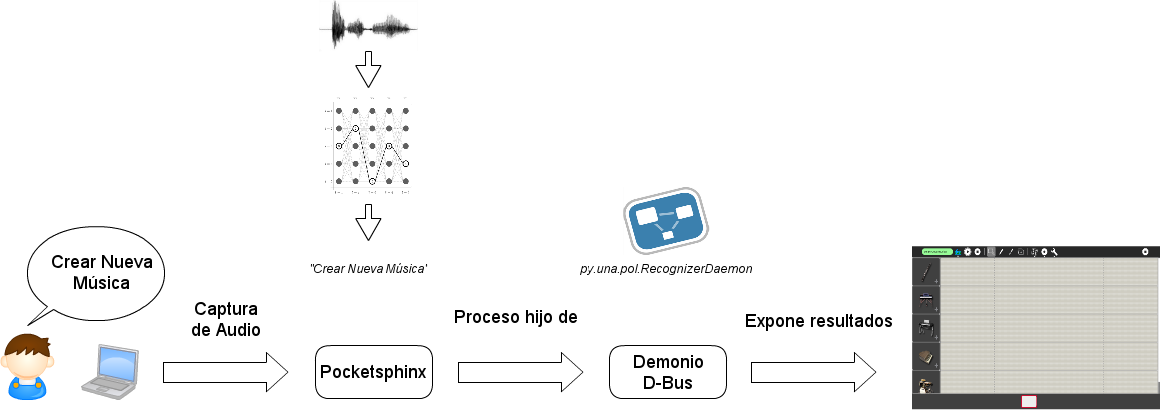
\includegraphics[width=1.0\textwidth]{./graphics/tamtam-proceso.png}
\caption{Arquitectura b\'asica de \emph{TamTam Listens}}
\label{figure:tamtam-listens-proceso}
\end{figure}

\subsection{Proceso del Reconocimiento del Habla}
\label{sec:proceso-solucion}

\foreign{PocketSphinx} implementa el proceso del reconocimiento del habla basado en el enfoque 
estad{\'\i}stico, el cual se present\'o en el cap{\'\i}tulo~\ref{sec:proceso}. La librer{\'\i}a incluye
los diferentes algoritmos necesarios para las fases del proceso.

\begin{figure}[H] 
\centering
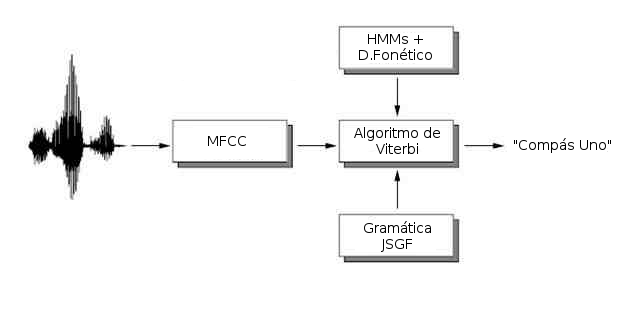
\includegraphics[width=0.8\textwidth]{./graphics/pocketsphinx.png}
\caption{Reconocimiento del habla mediante PocketSphinx. Gr\'afico basado en \cite{VerenichASR}.}
\label{figure:proceso-pocketsphinx}
\end{figure}

Como conjunto de caracter{\'\i}sticas espectrales, \foreign{Pocketsphinx} utiliza los coeficientes
espectrales en las frecuencias de mel (MFCC por sus siglas en ingl\'es).

En los \gls{hmm} del modelo ac\'ustico, utiliza mezclas Gaussianas para definir las probabilidades de 
transici\'on entre estados. El diccionario fon\'etico debe ser definido por el desarrollador.

Aunque \foreign{PocketSphinx} soporta modelos de lenguaje basados en n-gramas, para este trabajo 
se utiliza un modelo de lenguaje basado en gram\'atica. Esto se debe a la simpleza del lenguaje y a la 
falta de datos de entrenamiento para un modelo estad{\'\i}stico del mismo.

Como decodificador se utiliza el algoritmo de Viterbi, haciendo uso de la t\'ecnica de b\'usqueda en haz
para reducir el espacio de b\'usqueda.

Para hacer posible el reconocimiento del habla debe definirse el vocabulario que forma parte del 
dominio de la aplicaci\'on, su pronunciaci\'on y el conjunto de oraciones (en este caso, comandos 
v\'alidos) soportados por la aplicaci\'on. En otras palabras, \emph{Pocketsphinx} requiere un
modelo ac\'ustico y un modelo de lenguaje para funcionar.

\subsection{Modelo Ac\'ustico}
\label{sec:acustico-solucion}

El modelo ac\'ustico utilizado tiene como base las grabaciones de \foreign{Voxforge} en idioma espa\~nol,
y se encuentra disponible entre los recursos del proyecto \foreign{Pocketsphinx} para su utilizaci\'on
con el motor de reconocimiento del habla.

El diccionario fon\'etico define la secuencia de fonemas de cada palabra del lenguaje.
Este diccionario es utilizado por \emph{PocketSphinx} para asociar los fonemas reconocidos por
el modelo ac\'ustico a palabras v\'alidas del dominio de la aplicaci\'on.
En la figura~\ref{figure:fragmento-dic} se puede observar un fragmento del diccionario fon\'etico
utilizado por \emph{TamTam Listens}.

\lstset{
  basicstyle=\scriptsize,        % the size of the fonts that are used for the code
  breakatwhitespace=false,         % sets if automatic breaks should only happen at whitespace
  frame=single,                    % adds a frame around the code
  language=Octave,                 % the language of the code
  numbersep=5pt,                   % how far the line-numbers are from the code
  showstringspaces=false,          % underline spaces within strings only
  stepnumber=2,                    % the step between two line-numbers. If it's 1, each line will be numbered
  tabsize=2                       % sets default tabsize to 2 spaces
}

\begin{figure}[H]
\begin{lstlisting}
REPRODUCIR RR E P R O D U S I R
PAUSAR P A U S A R
PARAR  P A R A R
GENERAR  J E N E R A R
PARTITURA P A R T I T U R A
SIGUIENTE S I G I E N T E
ANTERIOR A N T E R I O R
\end{lstlisting}
\caption{Fragmento del diccionario fon\'etico utilizado en \emph{Tamtam Listens}.}
\label{figure:fragmento-dic}
\end{figure}

Como se puede observar, el formato del diccionario es bastante simple. Primero se define la palabra y 
a continuaci\'on los fonemas que la componen separados por espacios.
Una vez definidas las palabras de la aplicaci\'on, lo siguiente es determinar si una secuencia de
palabras es o no un comando v\'alido.

\subsection{Modelo de Lenguaje}
\label{sec:lenguaje-solucion}

Para el modelo de lenguaje se utiliza una gram\'atica en formato JSGF \cite{JSGF2000}, la cual permite
definir los comandos soportados por la aplicaci\'on de una manera sencilla.
En la figura~\ref{figure:fragmento-gram} puede observarse un fragmento de la gram\'atica utilizada por 
la aplicaci\'on.

\begin{figure}[H]
\begin{lstlisting}
#JSGF V1.0;
grammar tamtam;

public <tamtam-listens> = <comando> | <pagina> | <pista-a>     | <pista-b>  | 
                          <seleccionar-compas> | <crear-nota>  | <seleccionar-nota> | 
                          <duplicar-nota>      | <borrar-nota> | <volumen> | <tempo> | 
                          <configurar-nota>    | <loop>;

<comando>  = REPRODUCIR MUSICA  | PAUSAR MUSICA   | PARAR MUSICA | GENERAR MUSICA | 
             CREAR NUEVA MUSICA | EXPORTAR MUSICA | SALIR DE TAMTAM;
<pagina>   = ( CREAR NUEVA | DUPLICAR | LIMPIAR ) PARTITURA | PARTITURA <orden>;
<orden>    = ( ANTERIOR | SIGUIENTE );
<loop>   (COMODIN)+;
\end{lstlisting}
\caption{Fragmento de la gram\'atica utilizada en \emph{Tamtam Listens}.}
\label{figure:fragmento-gram}
\end{figure} 


\subsection{Palabras fuera del Vocabulario}
\label{sec:oov}

La pronunciaci\'on de palabras fuera del vocabulario ocurre frecuentemente en numerosas aplicaciones
del reconocimiento del habla, y es una fuente conocida de errores en el reconocimiento \cite{Bazzi00Modeling}.

De modo a minimizar la cantidad de errores como consecuencia de las palabras fuera del vocabulario,
\foreign{TamTam Listens} integra a su gram\'atica un modelo de palabra gen\'erica. Este componente se
define mediante el no terminal $<loop>$ de la figura \ref{figure:fragmento-gram}.

Un modelo de palabra gen\'erica admite cualquier palabra que pueda pronunciarse, es decir, permite
cualquier secuencia arbitraria de fonemas \cite{Bazzi00Modeling}. 
En el caso de \foreign{TamTam Listens}, el no terminal $<loop>$ corresponde a una o m\'as repeticiones del
terminal $COMODIN$.

A su vez, el terminal $COMODIN$ est\'a asociado a cada uno de los fonemas en el diccionario fon\'etico de
\foreign{TamTam Listens}, como se observa en la figura \ref{figure:fragmento-comodin}.

\begin{figure}[H]
\begin{lstlisting}
COMODIN   A
COMODIN(2)  B
COMODIN(3)  C
COMODIN(4)  CH
COMODIN(5)  D
\end{lstlisting}
\caption{Definici\'on parcial de COMODIN en el diccionario de \emph{Tamtam Listens}.}
\label{figure:fragmento-comodin}
\end{figure}

La combinaci\'on de los componentes presentados en este cap\'itulo hizo posible implementar el motor 
de reconocimiento del habla como servicio de \emph{D-Bus} y as\'i ofrecer \emph{TamTam Listens} como una 
interfaz alternativa a la propuesta por \emph{TamTam Edit}.

En el siguiente cap\'itulo se presenta la evaluaci\'on de la interfaz implementada, teniendo en cuenta 
aspectos t\'ecnicos y funcionales.